Dans ce chapitre, je vais détailler les différentes formations et apprentissages que j'ai suivis au cours de mon stage. Ces formations m'ont été recommandées par mon équipe pour améliorer mes compétences techniques et surmonter certains obstacles rencontrés dans le projet. D'autres initiatives ont été prises de mon propre chef pour mieux m'intégrer dans le domaine que je vise et démontrer mes capacités. L'objectif de ces formations était non seulement de résoudre les défis rencontrés durant le projet Audit365 Manager, mais aussi de renforcer ma compréhension globale des technologies et des pratiques pertinentes dans les domaines du \textbf{DevOps} et de l'\textbf{architecture cloud}, avec un accent particulier sur \textbf{Azure}.

\section{Certifications}

Durant mon stage, j'ai eu l'opportunité de me former et de passer des certifications essentielles pour approfondir mes connaissances dans les domaines de l'Azure et de Microsoft 365. Ces certifications, certaines déjà obtenues, ont non seulement renforcé ma compréhension des fondamentaux, mais ont également prouvé ma capacité à maîtriser des concepts complexes et à les appliquer de manière pratique. Dans cette section, je vais détailler les certifications que j'ai suivies, notamment Microsoft Azure Fundamentals AZ-900, Microsoft 365 Fundamentals MS-900, ainsi que la formation pour l'AZ-402. Chacune de ces certifications a été choisie pour répondre à des besoins spécifiques de mon projet et pour soutenir mon développement professionnel dans le domaine de l'architecture cloud et du DevOps.

\subsection{Microsoft Azure Fundamentals AZ-900}

Pour obtenir la certification \textbf{Microsoft Azure Fundamentals AZ-900}, j'ai suivi le parcours de formation proposé par Microsoft Learn. Ce parcours couvre les concepts fondamentaux du cloud computing, les services de base fournis par Azure, la gestion des coûts et la gouvernance. Les modules abordent également la sécurité, la confidentialité, la conformité et la confiance.

Voici un résumé des principales thématiques couvertes dans le parcours de Microsoft Learn :

\begin{itemize}
    \item[•] \textbf{Concepts de base du cloud} : Introduction aux principes fondamentaux du cloud computing, tels que l'élasticité, l'évolutivité et la résilience.
    \item[•] \textbf{Services principaux d'Azure} : Exploration des services Azure de base, y compris les machines virtuelles, le stockage, les bases de données et les réseaux.
    \item[•] \textbf{Sécurité et gouvernance} : Présentation des fonctionnalités de sécurité, des outils de gestion des identités et des stratégies de gouvernance pour garantir la conformité.
    \item[•] \textbf{Modèles de coût et de tarification} : Compréhension des différents modèles de tarification et des outils disponibles pour gérer les coûts sur Azure.
\end{itemize}

Ce parcours de formation m'a été particulièrement utile pour le projet \textbf{Audit365 Manager}, notamment pour la configuration de \textbf{Microsoft Entra ID}, où j'ai pu enregistrer des applications et gérer les identités et les accès de manière sécurisée.

En complément de ce parcours, je me suis également entraîné en ligne sur le site de Microsoft, qui propose des évaluations pratiques pour se préparer à l'examen. De plus, j'ai utilisé \href{https://www.examtopics.com/}{ExamTopics} pour m'entraîner avec des exemples de vraies questions d'examen, ce qui m'a aidé à mieux comprendre le format de l'examen et les types de questions posées.

Après avoir terminé la formation et les entraînements, j'ai passé l'examen et obtenu la certification \textbf{Microsoft Azure Fundamentals AZ-900}. Je suis très fier de cette réalisation, et l'entreprise l'a également bien accueillie. Étant en collaboration étroite avec Microsoft, l'entreprise encourage fortement ce type d'engagement et valorise les certifications qui renforcent nos compétences et notre expertise dans les technologies Microsoft.

\begin{figure}[H]
    \begin{center}
        \fbox{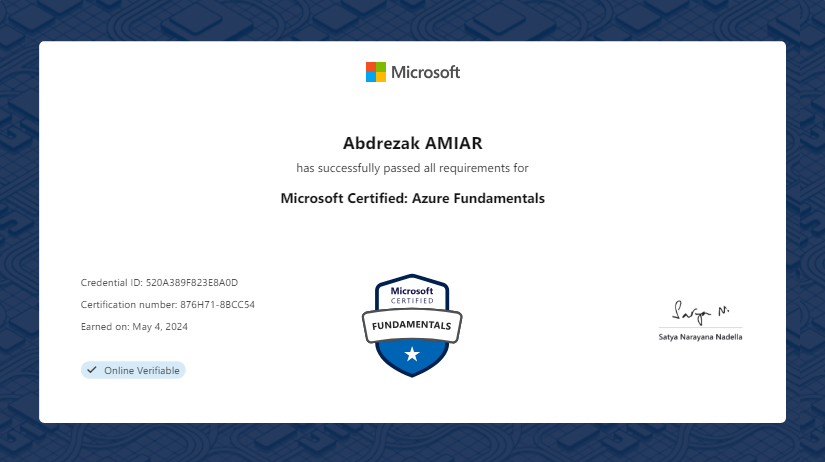
\includegraphics[scale=0.6]{images/MCAF.png}}
        \caption{Certification AZ-900}
    \end{center}
\end{figure}

\subsection{Microsoft365 Fundamentals MS-900}

j'ai suivi un parcours de formation similaire a celui de la premiere certification pour obtenir la \textbf{Microsoft 365 Fundamentals MS-900}. Ce parcours explore en profondeur les principaux concepts des services M365, les avantages de leur utilisation, ainsi que la gestion des utilisateurs et des identités. Les modules traitent également des aspects cruciaux tels que la sécurité, la conformité, la confidentialité et la gestion des abonnements.

Voici un résumé des principales thématiques abordées dans le parcours de Microsoft Learn :

\begin{itemize}
    \item[•] \textbf{Introduction à Microsoft 365} : Aperçu des services et des abonnements \textbf{M365}, avec un focus sur leurs avantages pour les entreprises.
    \item[•] \textbf{Productivité et collaboration} : Exploration des outils de collaboration comme \textbf{Teams}, \textbf{SharePoint} et \textbf{OneDrive}, ainsi que leur rôle dans le \textbf{Modern Workplace}.
    \item[•] \textbf{Gestion des identités et des accès} : Présentation des fonctionnalités de gestion des identités et des accès avec \textbf{Microsoft Entra ID} et les politiques de sécurité associées.
    \item[•] \textbf{Sécurité, conformité et confidentialité} : Discussion des outils et stratégies pour assurer la sécurité des données, la conformité aux normes et la confidentialité des informations dans Microsoft 365.
\end{itemize}

Grâce à ce parcours, j'ai acquis les compétences nécessaires pour auditer et gérer les services Microsoft 365, ce qui s'est avéré essentiel pour le projet \textbf{Audit365 Manager}. De plus, il m'a permis de m'intégrer efficacement à l'équipe en utilisant des outils de collaboration tels que \textbf{Teams} pour les communications, \textbf{Planner} pour la gestion des tâches, et \textbf{SharePoint} pour l'intranet d'entreprise.

Avec quelques entraînements, j'ai également pu obtenir ma deuxième certification, la \textbf{MS-900}.

\begin{figure}[H]
    \begin{center}
        \fbox{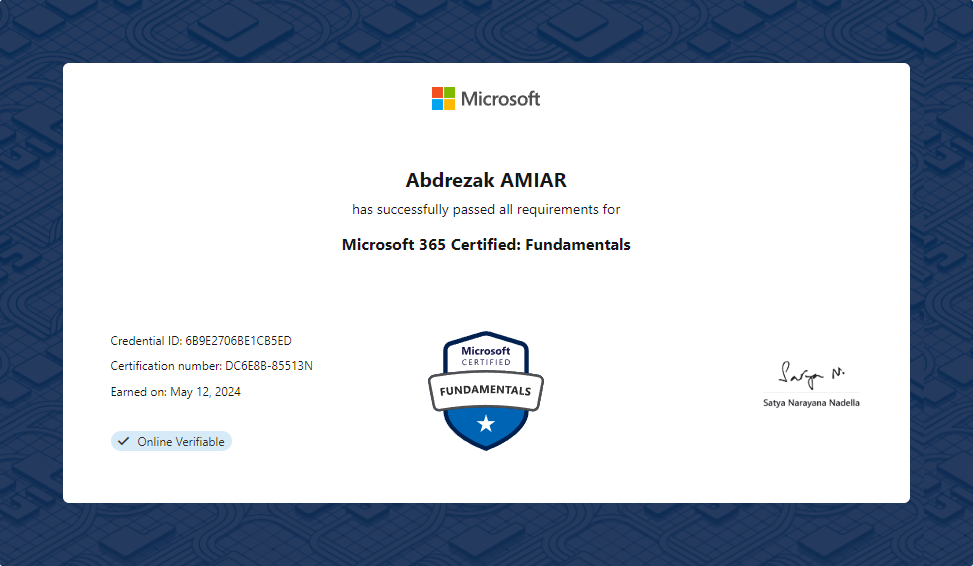
\includegraphics[scale=0.5]{images/MC365.png}}
        \caption{Certification MS-900}
    \end{center}
\end{figure}

\subsection{Microsoft Azure Developer Associate AZ-204}
J'ai récemment commencé la formation pour la certification \textbf{Microsoft Azure Developer Associate AZ-204} et je prévois de passer l'examen dans un futur proche. Cette formation s'est déjà avérée utile pour la conception de l'architecture du projet, en m'aidant à comprendre des concepts clés tels que les \textbf{web apps}, les \textbf{containers} et les \textbf{functions}.

\section{Formation en DevOps}
Dans cette section, je vais résumer la formations en \textbf{DevOps} que j'ai suivi pour renforcer mes compétences en \textbf{développement}, \textbf{intégration} et \textbf{déploiement} d'applications. Cette formation m'a permis de mieux comprendre et maîtriser les outils et pratiques \textbf{DevOps}, en particulier avec Azure DevOps. Bien que je n'aie pas encore eu l'occasion d'utiliser ces compétences dans le cadre du projet \textbf{Audit365 Manager}, car nous n'avons pas encore atteint la phase de déploiement et d'automatisation, je considère ces connaissances comme un atout précieux qui nous sera très utile dans un avenir proche.


\subsection{Qu'est-ce que le DevOps}

La formation \textbf{\href{https://learn.microsoft.com/en-us/training/paths/devops-foundations-core-principles-practices/}{DevOps Foundations: Core Principles and Practices}} couvre les concepts fondamentaux du DevOps, un ensemble de pratiques visant à automatiser et à intégrer les processus entre les équipes de développement et les opérations. Les principaux sujets abordés incluent les principes de collaboration, l'automatisation, l'intégration continue, la livraison continue, et la surveillance continue. Cette formation m'a aidé à comprendre comment ces pratiques peuvent améliorer la rapidité et la qualité des livraisons de logiciels, tout en réduisant les risques.

\subsection{Construction d’application avec Azure DevOps}

La formation \textbf{\href{https://learn.microsoft.com/en-us/training/paths/build-applications-with-azure-devops/}{Build Applications with Azure DevOps}} se concentre sur l'utilisation d'\textbf{Azure DevOps} pour planifier, développer et gérer des applications. Les principaux sujets incluent la gestion de projets avec Azure Boards, le contrôle de version avec Azure Repos, et la mise en place d'\textbf{intégrations continues (CI)} avec Azure Pipelines. Cette formation m'a permis de comprendre comment structurer et gérer efficacement des projets de développement en utilisant les outils \textbf{Azure DevOps}, même si je n'ai pas encore eu l'occasion de mettre ces compétences en pratique dans le cadre du projet actuel.

\subsection{Déploiement d’application avec Azure DevOps}

La formation \textbf{\href{https://learn.microsoft.com/en-us/training/paths/deploy-applications-with-azure-devops/}{Deploy Applications with Azure DevOps}} traite du déploiement et de la gestion des applications avec \textbf{Azure DevOps}. Les principaux sujets abordés incluent la création et l'exécution de pipelines de \textbf{déploiement continu (CD)}, la gestion des configurations de déploiement, et l'utilisation d'Azure Pipelines pour automatiser les déploiements. Cette formation m'a apporté une compréhension approfondie de la manière d'automatiser les processus de déploiement, de surveiller les applications en production, et de gérer les versions des applications de manière efficace et sécurisée. Ces compétences seront importantes pour la phase de déploiement de notre projet \textbf{Audit365 Manager}.

\section{Participation à un événement Microsoft sur les nouvelles technologies IA}

J'ai eu l'opportunité de participer à un événement organisé par Microsoft sur les nouvelles technologies en \textbf{intelligence artificielle (IA)}. Cet événement, intitulé "Créer des applications intelligentes avec Azure", s'est tenu au siège de Microsoft à Issy-les-Moulineaux. J'y ai passé la journée, profitant d'une session couvrante d'une variété de sujets sur les dernières avancées et applications de l'\textbf{IA}, offrant des perspectives précieuses sur l'impact de l'\textbf{IA} dans divers secteurs. La participation à cet événement m'a permis de mieux comprendre comment les technologies \textbf{IA} peuvent être intégrées dans les solutions d'entreprise pour améliorer l'efficacité et l'innovation.

\section{Formation sur les LLM (Large Language Models) chez Microsoft}

Au cours de cet événement, j'ai également suivi une introduction sur les \textbf{Large Language Models (LLM)} proposée par Microsoft. La formation s'est déroulée en deux parties : une session théorique le matin et une session pratique l'après-midi, guidée par des experts leaders dans le domaine de l'IA.

\subsection{Azure AI Studio}

La première partie de la formation portait sur l'\textbf{Azure AI Studio}, un outil puissant pour créer, entraîner et déployer des modèles d'intelligence artificielle. \textbf{Azure AI Studio} offre une interface intuitive pour travailler avec des modèles de langage, facilitant ainsi leur intégration dans diverses applications. J'ai appris à utiliser cet outil pour développer des solutions AI personnalisées, optimiser les performances des modèles et déployer des solutions AI à grande échelle.

\subsection{Prompt engineering}

La deuxième partie de la formation était axée sur le \textbf{prompt engineering}, une technique essentielle pour interagir efficacement avec les \textbf{LLM}. Le \textbf{prompt engineering} consiste à concevoir des entrées (\textbf{prompts}) optimisées pour obtenir des réponses précises et pertinentes des modèles de langage. J'ai acquis des compétences en création et ajustement de \textbf{prompts} pour différents cas d'utilisation, améliorant ainsi la qualité et la fiabilité des réponses générées par les \textbf{LLM}.

\subsection{Fine tuning}

Enfin, la formation a couvert le \textbf{fine tuning} des modèles de langage, une étape cruciale pour adapter les \textbf{LLM} aux besoins spécifiques d'une organisation. Le \textbf{fine tuning} implique l'ajustement des modèles pré-entraînés sur des données spécifiques à un domaine ou à une application, afin d'améliorer leur performance et leur pertinence. J'ai appris les techniques de \textbf{fine tuning} et comment les appliquer pour optimiser les \textbf{LLM} pour des tâches précises, augmentant ainsi leur utilité et leur efficacité dans des contextes réels.

L'après-midi, j'ai eu l'occasion de mettre en pratique ces connaissances sous la direction des leaders experts présents.Durant cette session, j'ai eu l'opportunité de mettre en œuvre concrètement les concepts appris le matin. J'ai commencé par déployer des modèles IA avancés tels que \textbf{GPT-3.5} et \textbf{GPT-4} en utilisant Azure AI Studio. Cela m'a permis de comprendre les nuances et les paramètres nécessaires pour optimiser le déploiement de ces modèles. J'ai ensuite exploré les techniques de \textbf{prompt engineering}, où j'ai appris à structurer et formuler des prompts pour obtenir des réponses plus précises et pertinentes des modèles IA. Un aspect particulièrement enrichissant de la session pratique a été le \textbf{prompt flow}. En ajustant les prompts et en expérimentant avec différents scénarios, j'ai pu voir comment de petites modifications pouvaient grandement influencer les résultats produits par les modèles. Cette expérience m'a également sensibilisé à l'importance du contexte et de la clarté dans la formulation des prompts.


Bien que cette formation n'était qu'une introduction au monde de l'\textbf{IA}, elle m'a équipé des connaissances et des compétences de base nécessaires pour commencer à exploiter le potentiel des \textbf{Large Language Models} dans des environnements professionnels. Cela renforce ma capacité à contribuer à des projets innovants dans le domaine de l'\textbf{intelligence artificielle}.

\section{Portfolio Website}

Au cours de mon temps libre, notamment les week-ends et plusieurs jours fériés du mois de mai, j'ai développé mon propre site web personnel, \textbf{\href{https://www.amiar.fr/}{www.amiar.fr}}. Ce projet m'a permis de mettre en pratique les connaissances acquises en développement web et en déploiement sur le cloud \textbf{Azure}.

Grâce aux compétences acquises durant les différentes formations et expériences de stage, notamment en \textbf{Azure}, j'ai pu créer et déployer mon site web avec une grande facilité. Le site présente mon parcours, mes compétences et mes projets, offrant une vitrine professionnelle de mon travail.

Le développement du site m'a permis d'utiliser diverses technologies apprises pendant le stage, telles que :

\begin{itemize}
    \item[•] \textbf{HTML, CSS, et JavaScript} : Pour construire et styliser les pages web.
    \item[•] \textbf{Azure Storage et Azure Custom Domain Name (CDN)} : Pour héberger et distribuer les contenus de manière efficace.
    \item[•] \textbf{Azure Front Door} : Pour sécuriser et optimiser l'accès au site web.
\end{itemize}

En outre, les connaissances acquises à l'université ont également joué un rôle important dans ce projet. Les bases solides en programmation et en développement web que j'ai obtenues durant mes études m'ont permis d'aborder ce projet avec confiance et compétence.

Le processus de déploiement sur Azure a été grandement facilité par les connaissances acquises lors de mes formations et de mon travail sur le projet Audit365 Manager. J'ai déployé et configuré un \textbf{Azure Storage} puis activé une page web statique. J'ai ensuite déposé les fichiers de la page web dans un conteneur du stockage, rendant mon site disponible. Pour améliorer la sécurité et permettre un nom de domaine personnalisé (\textbf{CDN}), j'ai configuré un \textbf{Azure Front Door}, hébergeant ainsi mon site web sur \href{https://www.amiar.fr/}{wwW.amiar.fr}.


Ce projet personnel m'a non seulement permis de consolider mes compétences techniques, mais aussi de créer un outil précieux pour ma carrière professionnelle. Il démontre ma capacité à appliquer les technologies apprises dans des projets concrets et à contribuer de manière significative à des initiatives technologiques.

\begin{figure}[H]
    \begin{center}
        \fbox{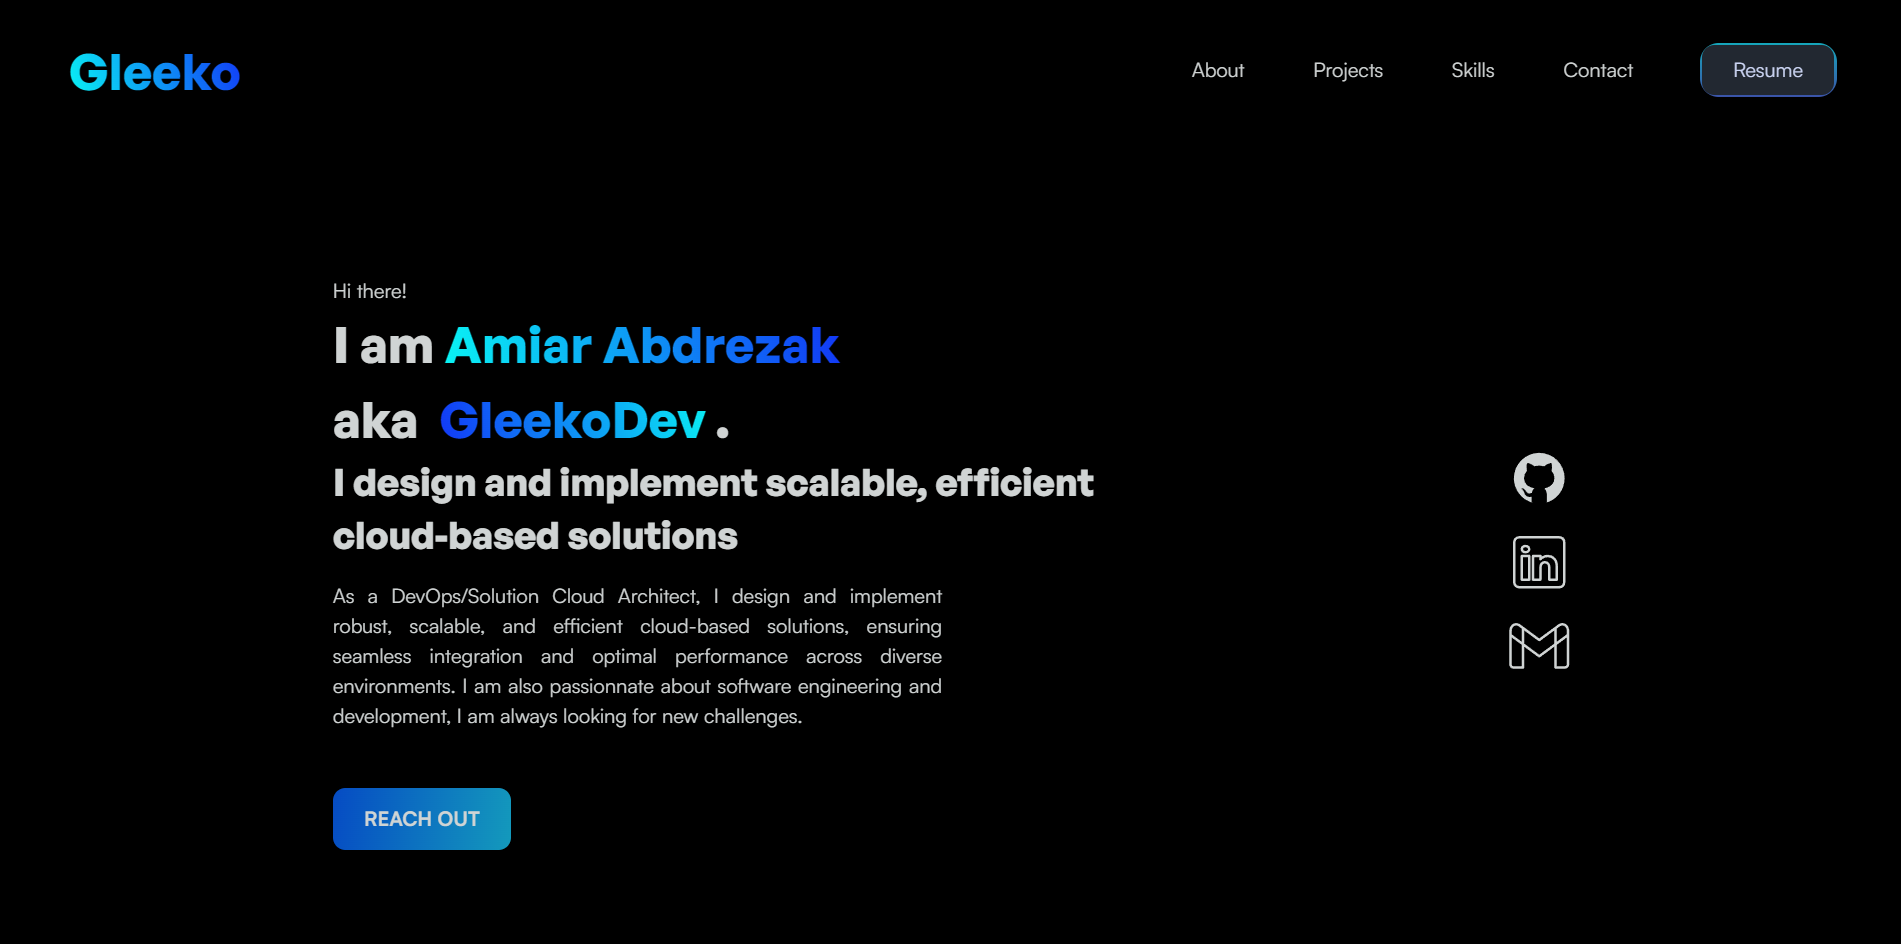
\includegraphics[scale=0.37]{images/webportfolio.png}}
        \caption{Site Vitrine de Amiar Abdrezak}
    \end{center}
\end{figure}


\section{Résumé des apprentissages}

Au cours de mon stage, j'ai eu l'opportunité d'acquérir et de consolider un large éventail de compétences techniques et pratiques. Voici un résumé des principales technologies et outils que j'ai appris et utilisés :

\begin{itemize}
    \item[•] \textbf{Azure} : Utilisation des services Azure tels que Azure Storage, Azure CDN, Azure Front Door, Web Apps, Functions et la gestion des ressources dans le portail Azure.
    \item[•] \textbf{PowerShell} : Développement de scripts pour automatiser les tâches, gestion des configurations et réalisation des audits.
    \item[•] \textbf{C\#} : Programmation en C\# pour le développement d'applications.
    \item[•] \textbf{Microsoft 365} : Utilisation et gestion des services comme SharePoint, Teams, OneDrive et la suite Microsoft 365 dans son ensemble.
    \item[•] \textbf{Planner et méthodes Agile} : Gestion des tâches et des projets, suivi des progrès à l'aide des tableaux Kanban, et application des principes Agile pour une gestion de projet efficace.
    \item[•] \textbf{DevOps} : Compréhension des principes de DevOps, création et gestion des pipelines CI/CD, et utilisation de Azure DevOps pour le déploiement des applications.
    \item[•] \textbf{HTML, CSS et JavaScript} : Développement et stylisation de pages web.
    \item[•] \textbf{Fiddler} : Utilisation pour la surveillance et l'analyse des flux de données pour assurer la sécurité des applications.
    \item[•] \textbf{Azure AI Studio} : Utilisation pour les projets impliquant des modèles de langage étendus (LLM).
    \item[•] \textbf{LLM (Large Language Models)} : Formation sur les grands modèles de langage et leur application ainsi que sur le Prompt Engineering et le Fine Tuning.
\end{itemize}

Ces apprentissages m'ont permis de développer une compréhension approfondie des technologies cloud et des pratiques de DevOps, de renforcer mes compétences en développement web et d'acquérir une expérience précieuse en gestion de projets et en collaboration au sein d'une équipe. L'application des méthodes Agile, en particulier, a été essentielle pour structurer notre travail et garantir une communication fluide et une adaptation rapide aux changements. Ces compétences seront essentielles pour ma carrière future et m'aideront à contribuer efficacement à des projets technologiques complexes.
